% VUT FIT MITAI
% MSZ 2021/2022
% Author: Vladimir Dusek
% Login: xdusek27

%%%%%%%%%%%%%%%%%%%%%%%%%%%%%%%%%%%%%%%%%%%%%%%%%%%%%%%%%%%%%%%%%%%%%%%%%%%%%%%%

% Path to figures
\graphicspath{{tin/nerozhodnutelnost/figures}}

%%%%%%%%%%%%%%%%%%%%%%%%%%%%%%%%%%%%%%%%%%%%%%%%%%%%%%%%%%%%%%%%%%%%%%%%%%%%%%%%

\chapter{TIN~--~Nerozhodnutelnost (problém zastavení TS, princip diagonalizace a redukce, Postův korespondenční problém).}

%%%%%%%%%%%%%%%%%%%%%%%%%%%%%%%%%%%%%%%%%%%%%%%%%%%%%%%%%%%%%%%%%%%%%%%%%%%%%%%%

\section{Zdroje}

\begin{compactitem}
    \item \path{tin_2021_merged.pdf}
    \item \path{TIN_todo.mp4}
\end{compactitem}

%%%%%%%%%%%%%%%%%%%%%%%%%%%%%%%%%%%%%%%%%%%%%%%%%%%%%%%%%%%%%%%%%%%%%%%%%%%%%%%%

\section{Rozhodovací problém}

Jakýkoliv rozhodovací problém, dokážeme kódovat na jazyk. Více TS 2, slajd 3/19. \todo{todo}

Nechť $P$ je problém specifikovaný jazykem $L_P$ nad abecedou $\Sigma$. Problém P nazveme: \begin{compactitem}

    \item \textbf{Rozhodnutelný}, pokud $L_P$ je rekurzívní jazyk, tj. existuje TS, který $L_P$ rozhoduje (přijme každý řetězec $w \in L_P$, a zamítne každý řetězec $w \in \Sigma^* - L_P $).

    \item \textbf{Nerozhodnutelný}, když není rozhodnutelný.

    \item \textbf{Částečně rozhodnutelný}, jestliže LP je rekurzívně vyčíslitelný jazyk.

\end{compactitem}

Každý rozhodnutelný problém je současně částečně rozhodnutelný, ale některé nerozhodnutelné problémy nejsou ani částečně rozhodnutelné.

Problém je nerozhodnutelný, pokud pro něj neexistuje úplný turingův stroj.

Zjistit jestli turingův stroj je úplný, je taky problém.

\begin{figure}[H]
    \centering
    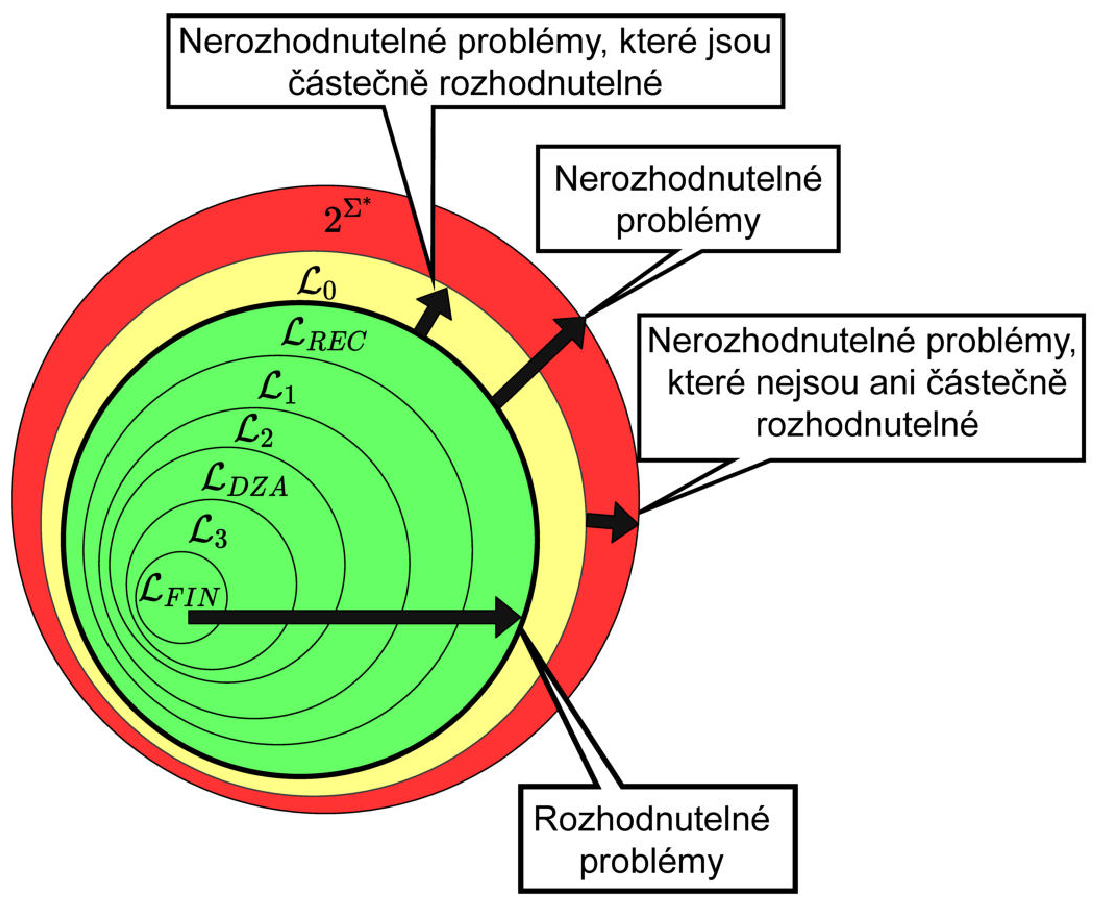
\includegraphics[width=0.9\linewidth]{fj_hierarchy.pdf}
    \caption{Hierarchie.}
\end{figure}

\paragraph*{Halting Problem} Problém zastavení turingova stroje.

$$ HP = \{ \langle M \rangle \# \langle w \rangle ~|~ \text{TS M na vstupu w zastaví} \} $$

\paragraph*{co-Halting Problem} Problém nezastavení turingova stroje.

$$ coHP = \{ \langle M \rangle \# \langle w \rangle ~|~ \text{TS M na vstupu w nezastaví} \} $$

%%%%%%%%%%%%%%%%%%%%%%%%%%%%%%%%%%%%%%%%%%%%%%%%%%%%%%%%%%%%%%%%%%%%%%%%%%%%%%%%

\section{Diagonalizace}

Spočetné -- umím spočítat a uspořádat. Existuje bijekce mezi množinou N a každou spočetnou množinou. Dokážu namapovat.

Jazyků je nespočetně mnoho.

Ale všech možný programů (TS) je spočetně mnoho, proč? Protože kódování TS je možné interpretovat jako přirozené číslo. A těch je spočetně mnoho.

\todo{todo}

todo dukaz Existence jazyků mimo třídu 0

K porovnávání mohutnosti dvou množin

%%%%%%%%%%%%%%%%%%%%%%%%%%%%%%%%%%%%%%%%%%%%%%%%%%%%%%%%%%%%%%%%%%%%%%%%%%%%%%%%

\section{Redukce}

\begin{compactitem}

    \item Problém je aspoň tak těžkej jako problém

    \item Vytváří uspořádání na problémech, nějaký problém je aspoň tak těžký jak jiný problém

    \item Redukce jazyka A na jazyk B je totální, rekurzivně vyčíslitelná funkce... (To znamená, že je implementovatelné pomocí úplného TS)

    \item Zachovává členství.

    \item Existuje-li redukce jazyka $A$ na $B$, říkáme, že $A$ je redukovatelný na $B$, což značíme $A \leq B$.

\end{compactitem}


\todo{todo}

%%%%%%%%%%%%%%%%%%%%%%%%%%%%%%%%%%%%%%%%%%%%%%%%%%%%%%%%%%%%%%%%%%%%%%%%%%%%%%%%

\section{Postův korespondenční problém}

\todo{todo}
